\documentclass[14pt]{extbook}
\usepackage{multicol, enumerate, enumitem, hyperref, color, soul, setspace, parskip, fancyhdr} %General Packages
\usepackage{amssymb, amsthm, amsmath, latexsym, units, mathtools} %Math Packages
\everymath{\displaystyle} %All math in Display Style
% Packages with additional options
\usepackage[headsep=0.5cm,headheight=12pt, left=1 in,right= 1 in,top= 1 in,bottom= 1 in]{geometry}
\usepackage[usenames,dvipsnames]{xcolor}
\usepackage{dashrule}  % Package to use the command below to create lines between items
\newcommand{\litem}[1]{\item#1\hspace*{-1cm}\rule{\textwidth}{0.4pt}}
\pagestyle{fancy}
\lhead{Progress Quiz 8}
\chead{}
\rhead{Version C}
\lfoot{5493-4176}
\cfoot{}
\rfoot{Summer C 2021}
\begin{document}

\begin{enumerate}
\litem{
First, find the equation of the line containing the two points below. Then, write the equation in the form $ y=mx+b $ and choose the intervals that contain $m$ and $b$.\[ (-5, -7) \text{ and } (-7, 9) \]\begin{enumerate}[label=\Alph*.]
\item \( m \in [-12, -6] \hspace*{3mm} b \in [44, 52] \)
\item \( m \in [-12, -6] \hspace*{3mm} b \in [16, 22] \)
\item \( m \in [-12, -6] \hspace*{3mm} b \in [-52, -46] \)
\item \( m \in [5, 12] \hspace*{3mm} b \in [62, 72] \)
\item \( m \in [-12, -6] \hspace*{3mm} b \in [-6, 6] \)

\end{enumerate} }
\litem{
Solve the equation below. Then, choose the interval that contains the solution.\[ -5(-19x + 6) = -11(14x + 18) \]\begin{enumerate}[label=\Alph*.]
\item \( x \in [-3.99, -3.73] \)
\item \( x \in [0.91, 1.45] \)
\item \( x \in [-0.83, -0.37] \)
\item \( x \in [-1.35, -0.74] \)
\item \( \text{There are no real solutions.} \)

\end{enumerate} }
\litem{
Write the equation of the line in the graph below in Standard Form $Ax+By=C$. Then, choose the intervals that contain $A, B, \text{ and } C$.
\begin{center}
    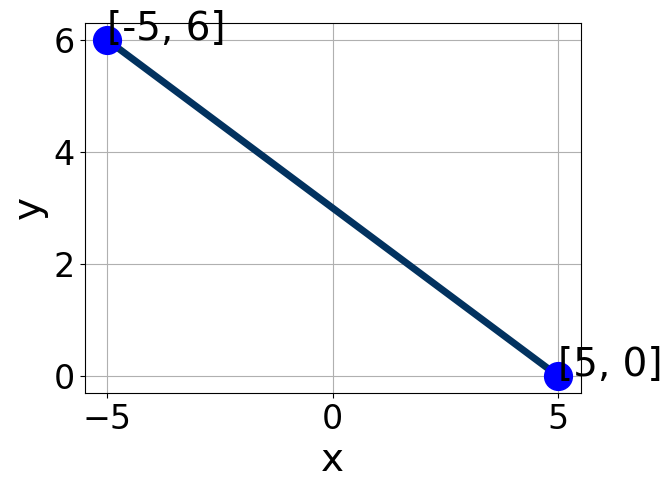
\includegraphics[width=0.5\textwidth]{../Figures/linearGraphToStandardC.png}
\end{center}
\begin{enumerate}[label=\Alph*.]
\item \( A \in [-1.1, 1], \hspace{3mm} B \in [-2.6, 0], \text{ and } \hspace{3mm} C \in [-6, -2] \)
\item \( A \in [2.9, 4.4], \hspace{3mm} B \in [-5.1, -4], \text{ and } \hspace{3mm} C \in [-20, -4] \)
\item \( A \in [-7.6, 0.5], \hspace{3mm} B \in [-5.1, -4], \text{ and } \hspace{3mm} C \in [-20, -4] \)
\item \( A \in [2.9, 4.4], \hspace{3mm} B \in [3.1, 6.3], \text{ and } \hspace{3mm} C \in [12, 19] \)
\item \( A \in [-1.1, 1], \hspace{3mm} B \in [0.5, 2.7], \text{ and } \hspace{3mm} C \in [3, 5] \)

\end{enumerate} }
\litem{
Find the equation of the line described below. Write the linear equation in the form $ y=mx+b $ and choose the intervals that contain $m$ and $b$.\[ \text{Perpendicular to } 5 x - 3 y = 15 \text{ and passing through the point } (5, 4). \]\begin{enumerate}[label=\Alph*.]
\item \( m \in [-0.67, -0.16] \hspace*{3mm} b \in [-7.6, -3.6] \)
\item \( m \in [-0.67, -0.16] \hspace*{3mm} b \in [6.5, 9.2] \)
\item \( m \in [-0.67, -0.16] \hspace*{3mm} b \in [-2, -0.9] \)
\item \( m \in [0.54, 1.76] \hspace*{3mm} b \in [0.2, 1.3] \)
\item \( m \in [-1.98, -1.35] \hspace*{3mm} b \in [6.5, 9.2] \)

\end{enumerate} }
\litem{
Solve the linear equation below. Then, choose the interval that contains the solution.\[ \frac{8x + 3}{7} - \frac{-3x + 8}{4} = \frac{7x + 4}{3} \]\begin{enumerate}[label=\Alph*.]
\item \( x \in [-21.5, -19.9] \)
\item \( x \in [1.5, 4.4] \)
\item \( x \in [-0.4, 1.7] \)
\item \( x \in [-7.1, -4.1] \)
\item \( \text{There are no real solutions.} \)

\end{enumerate} }
\litem{
Find the equation of the line described below. Write the linear equation in the form $ y=mx+b $ and choose the intervals that contain $m$ and $b$.\[ \text{Parallel to } 8 x + 9 y = 9 \text{ and passing through the point } (6, 4). \]\begin{enumerate}[label=\Alph*.]
\item \( m \in [-1, 0.3] \hspace*{3mm} b \in [-2.73, -1.89] \)
\item \( m \in [-1.3, -0.9] \hspace*{3mm} b \in [9.04, 9.97] \)
\item \( m \in [-0.3, 2.8] \hspace*{3mm} b \in [-1.84, -0.93] \)
\item \( m \in [-1, 0.3] \hspace*{3mm} b \in [-10.03, -8.99] \)
\item \( m \in [-1, 0.3] \hspace*{3mm} b \in [9.04, 9.97] \)

\end{enumerate} }
\litem{
Solve the equation below. Then, choose the interval that contains the solution.\[ -13(-16x -2) = -9(10x + 5) \]\begin{enumerate}[label=\Alph*.]
\item \( x \in [0.1, 0.21] \)
\item \( x \in [0.03, 0.14] \)
\item \( x \in [-0.26, -0.15] \)
\item \( x \in [-0.18, 0] \)
\item \( \text{There are no real solutions.} \)

\end{enumerate} }
\litem{
First, find the equation of the line containing the two points below. Then, write the equation in the form $ y=mx+b $ and choose the intervals that contain $m$ and $b$.\[ (7, -2) \text{ and } (-9, 3) \]\begin{enumerate}[label=\Alph*.]
\item \( m \in [-0.44, 0.04] \hspace*{3mm} b \in [-0.1, 1.7] \)
\item \( m \in [0.18, 0.4] \hspace*{3mm} b \in [4.48, 6.93] \)
\item \( m \in [-0.44, 0.04] \hspace*{3mm} b \in [-1.68, -0.09] \)
\item \( m \in [-0.44, 0.04] \hspace*{3mm} b \in [11.59, 12.01] \)
\item \( m \in [-0.44, 0.04] \hspace*{3mm} b \in [-9.78, -8.62] \)

\end{enumerate} }
\litem{
Write the equation of the line in the graph below in Standard Form $Ax+By=C$. Then, choose the intervals that contain $A, B, \text{ and } C$.
\begin{center}
    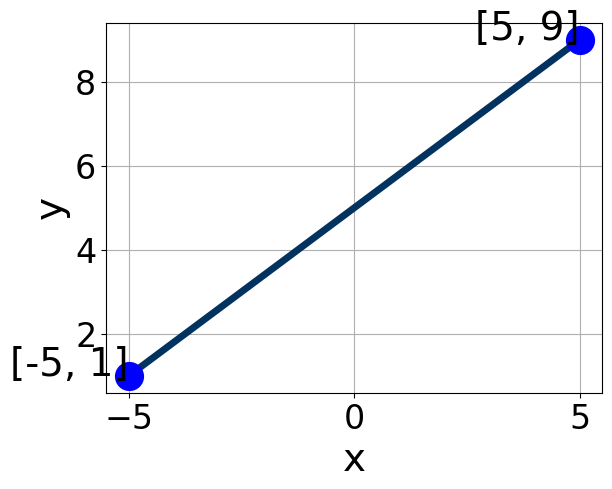
\includegraphics[width=0.5\textwidth]{../Figures/linearGraphToStandardCopyC.png}
\end{center}
\begin{enumerate}[label=\Alph*.]
\item \( A \in [-5.1, -3.9], \hspace{3mm} B \in [3.46, 5.47], \text{ and } \hspace{3mm} C \in [24, 29] \)
\item \( A \in [-3.8, 1.1], \hspace{3mm} B \in [-2.36, -0.99], \text{ and } \hspace{3mm} C \in [-6, -4] \)
\item \( A \in [-3.8, 1.1], \hspace{3mm} B \in [0, 1.29], \text{ and } \hspace{3mm} C \in [3, 7] \)
\item \( A \in [2.9, 7.6], \hspace{3mm} B \in [-5.22, -4.47], \text{ and } \hspace{3mm} C \in [-26, -17] \)
\item \( A \in [2.9, 7.6], \hspace{3mm} B \in [3.46, 5.47], \text{ and } \hspace{3mm} C \in [24, 29] \)

\end{enumerate} }
\litem{
Solve the linear equation below. Then, choose the interval that contains the solution.\[ \frac{-3x + 5}{2} - \frac{-6x + 9}{4} = \frac{-4x + 6}{5} \]\begin{enumerate}[label=\Alph*.]
\item \( x \in [0.2, 1.4] \)
\item \( x \in [10.7, 13.8] \)
\item \( x \in [-0.7, 0.2] \)
\item \( x \in [-5.1, -3.7] \)
\item \( \text{There are no real solutions.} \)

\end{enumerate} }
\end{enumerate}

\end{document}